%%%Preamble
% packages and document class
\documentclass[a4paper, 12pt]{article}
\usepackage[utf8]{inputenc}
\usepackage{geometry}
\usepackage{authblk}
\usepackage{lineno}
\usepackage{graphicx}

\bibliography{master_mutantag.bib}

% page format
\geometry{left = 3cm, top = 3cm, bottom = 2cm, right = 2cm}
\linespread{2.0}

% article basic infos
 \title{\line(1,0){250}\\From mutualism to antagonism: the coevolutionary influence of  context-dependent interactions in mutualistic networks\\\line(1,0){250}}

\author[1]{Lucas A. Camacho}
\author[2]{Paulo Roberto Guimarães Junior}
\date{}
\affil[1,2]{Departamento de Ecologia, Universidade de São Paulo, Rua do Matão, travessa 14, nº 321, Cidade Universitária, São Paulo - SP, CEP: 05508-090, Brasil.}

%%%Document begins
\begin{document}
\maketitle

\section{Introduction}
\linenumbers
Coevolution, the reciprocal evolutionary change between interacting species, is a main force influencing the diversity of species and the organization of ecological interactions in the community. The interactions structure (who interacts with whom) dictates which species are coevolving in the community. Thus, coevolution is a process that molds and is molded by ecological interactions. The most conspicuous known patterns of coevolution are on species traits related to ecological interactions like plants and herbivores, pollination or seed dispersal.

Historically, the empirical evidences of coevolution thrilled several worldwide known naturalists to describe the genetic and ecological mechanisms that fuel coevolution and, consequently, influences the ecological interactions between species in communities. Daniel Janzen described a high specialized mutualistic interaction formed by coevolution between the acacia ant (\textit{Pseudomyrmex ferruginea}) and the bullhorn acacia (\textit{Acacia cornigera}). In this system, the ant lives exclusively inside de acacia plant, repealing possible herbivores that may attack the plants. In this way, the ant has his colony guaranteed and the plant repeal unwanted visitors. Also, Fritz Müller studied the coloration patterns of neotropical butterflies and propose the first mathematical model to show how these patterns emerge in this butterflies by coevolution.

Systems of coevolution between two species  grounded the studies of how several species can coevolve in nature. Several species implies in several reciprocal evolutionary changes happening at the same time. Thus, coevolution process depends on how the ecological interactions are distributed in the community. A problem that emerge is how to account several reciprocal evolutionary changes at once. An possible approach to solve this issue is use network theory. Networks are representations of species and the interactions between these species in the community. The use of networks of interactions enable the investigation of how different evolutive process form phenotipic pattern of species. Using the networks approach, we now know that coevolution in mutualistic networks of interactions lead to trait complementarity of species that interact. In antagonisms otherwise, the selection intensity acting on a prey and the predator can create coevolutionary arm's race. This different coevolutionary dynamics can reorganize the interactions structure in time, generating for example, temporal variation in species traits between interacting species.

The species traits that will be favoured by natural selection, the interaction network structure and the path of the coevolution process rely on the costs and benefits associated with different interaction outcomes. For example, mutualisms shows a higher benefit compared to the cost for both interacting species. If so, the efficiency of interaction will be higher in species with similar traits, where  the specie that has the higher proportion of  interactions will order the trait complementarity generating a particular coevolution process. Else, antagonism interactions shows a higher benefit than the cost for a predator or parasite and a low benefit than the cost for the prey or host. Considering now an antagonism network of interactions, explorer species that has similar traits of explored species will be favoured, creating an arm's race coevolution dynamics. Despite the actual knowing of how these interaction outcomes will influence coevolution, there is a lack of knowledge on how these two otcomes in the same network can influence the coevolution process.


Despite the utility of using the interactions by their costs and benefits, these costs and benefits are not fixed. The variation of benefits and costs happens on the biotic and abiotic which the species are under. The interactions outcomes which vary because of biotic and abiotic factors are called context-dependent interactions.

There is growing evidence quantifying the outcomes variation of interactions in space and time. For example, mirmecophyte plants has structures called domatia and extrafloral nectaries which atract ants. These ants repeal natural enemies of plants like herbivores. But, a low abundance of ants caused by external factors of the plant can cause a low repealing efficiency from ants. In this scenario, is possible that the production cust of domatia and extrafloral nectaries for the plant could be lower than the benefits gived by the ants, for the low efficiency in repealing natural enemys of these ants. In this way, the interaction between mirmecophyte plants and ants can pass from a mutualism to an antagonism, which the ant is beneficied and the plant suffers from a higher cust, depending on the ecological context.

Depending on the interaction, this interaction outcome shift from mutualism to antagonism can happen in time. In this way, the "come and go" of mutualists and antagonism oucomes in a community result in coevolutionary dynamics favored by these two types of interactions. Both dynamics in the same community can influence species more in a mutualism or antagonism-like dynamic. In other words, the context dependency of interactions changing the interactions outcomes generates changes in the coevolutionary dynamics of species. In a general view, ecological interactions outcomes varying in space and time can change the coevolutive process, contributing to the trait diversity of species and interaction structure of the community. Finally, context-dependent interactions should not be ignored if we want a higher understanding of the ecossistems function and diversity. 

Here, we use a mathematical model, theoretical and empirical networks of species interactions and computer simulations to fill this gap. Especifically, we are trying to understand: \textit{i)} how changes the structure of networks of interactions with both antagonism and mutualism together? \textit{ii)} how context-dependent interactions influences the coevolutionary process?

% add figure 1
\begin{figure}
\linespread{1.0}
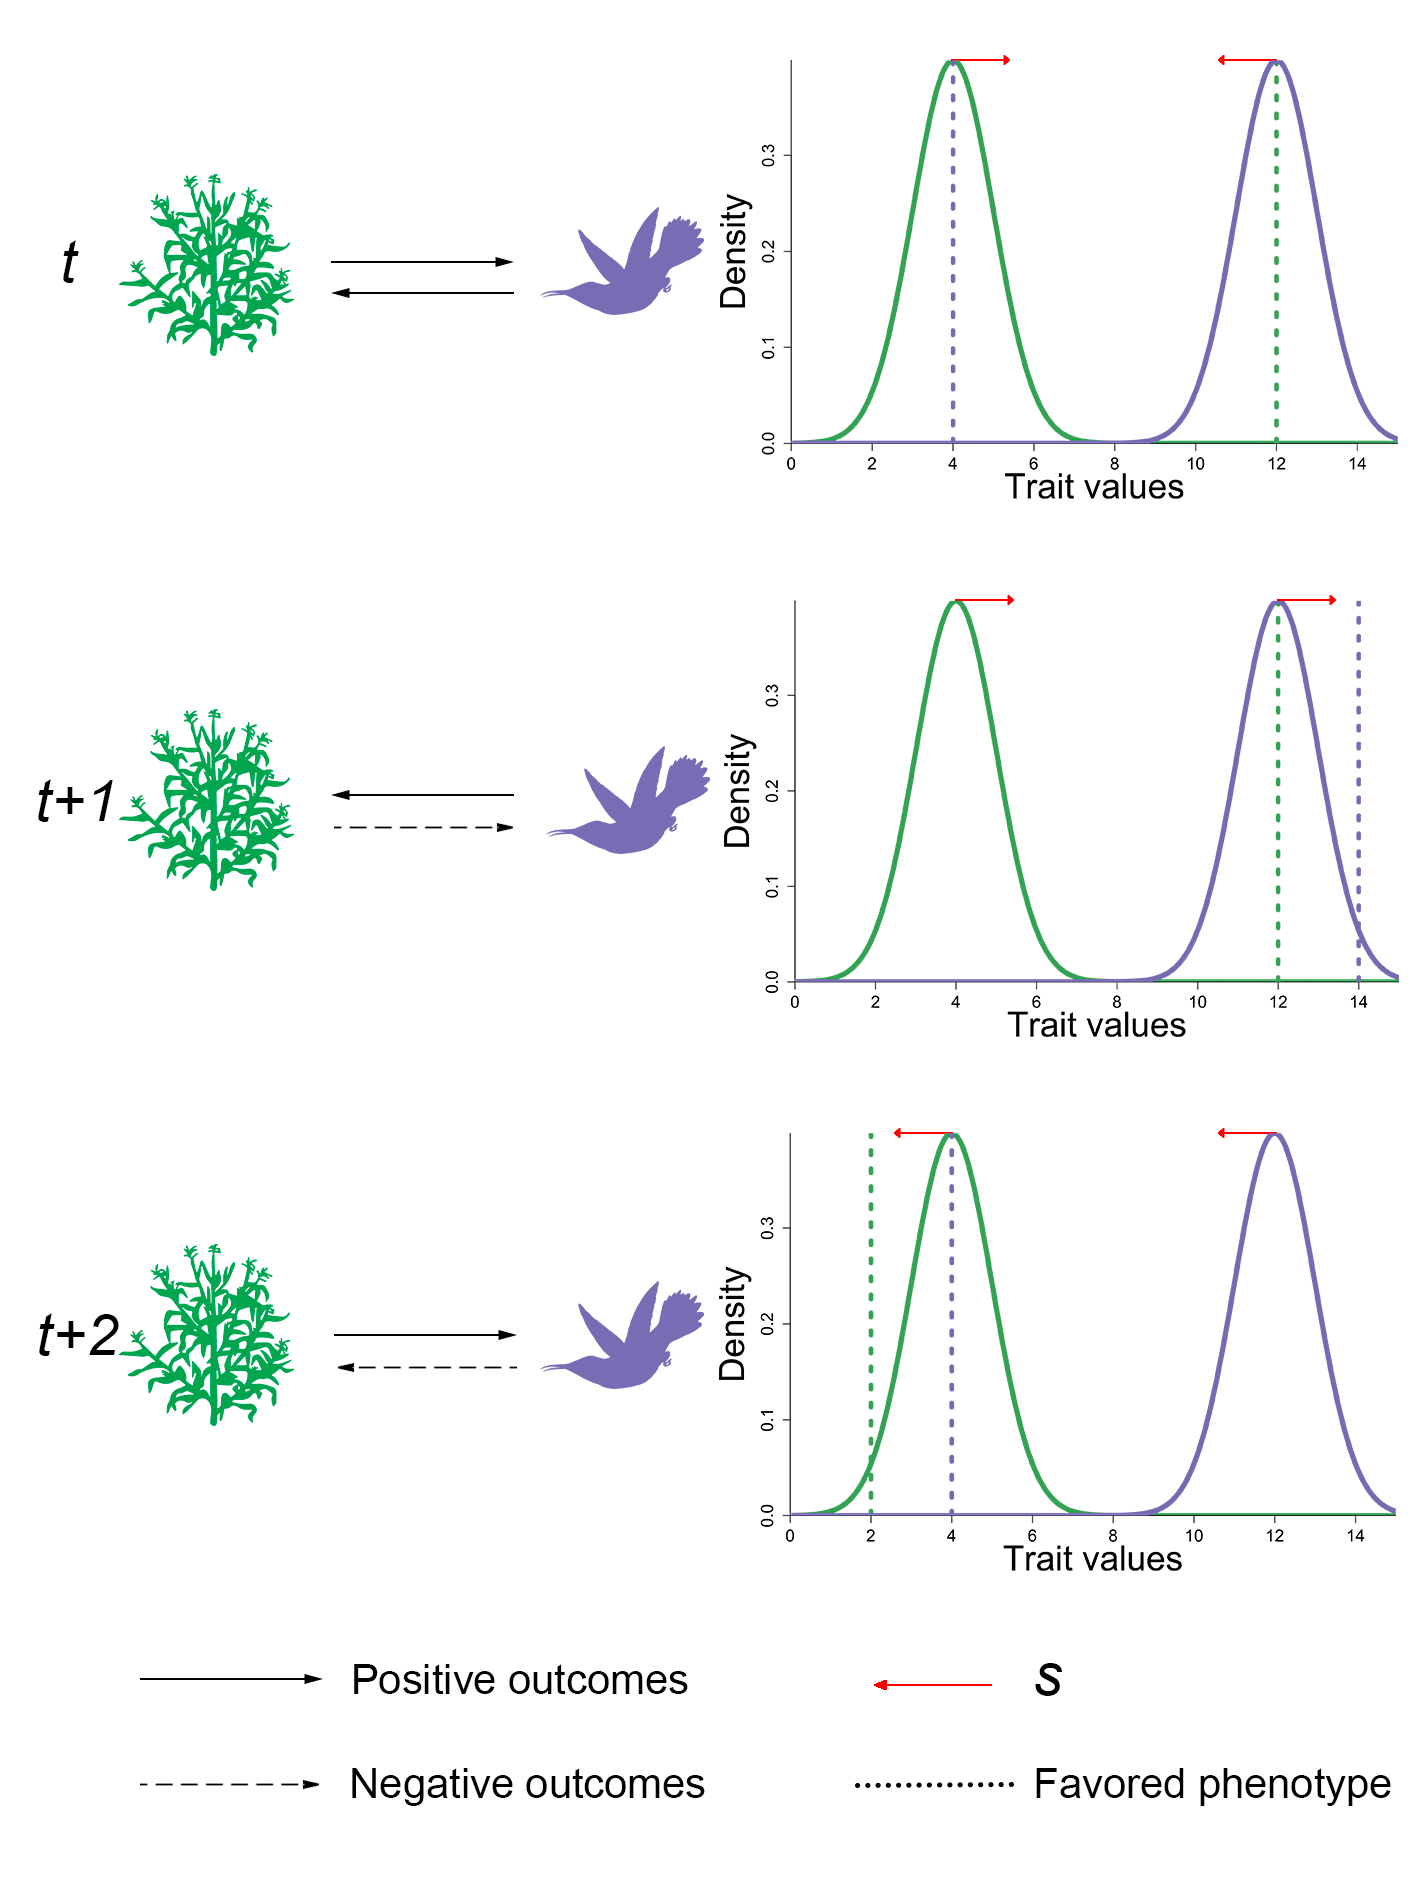
\includegraphics[width=\textwidth]{Fig1_ConDep.png}
\caption{Conceptual figure showing the interaction outcomes changing from a mutualism (t) to an antagonism with different outcome arrangements (t+1 and t+2). There are different favoured phenotypes and selection differentials (s) depending on how the interaction outcomes are arranged. The mutualism promotes trait matching and the antagonism promotes arm's race between the explorer and exploited species.}
\label{fig1}
\end{figure}

\nolinenumbers
\section{References}


\end{document}